
Our main outcome measures are the severity of the largest drop in the price of each cryptocoin, and the magnitude (volume) of the transactions made with the cryptocoin measured in USD.
We operationalize the intensity of a bubble as the proportion of a 1 dollar that would be lost buying at the maximum price and selling after that proportionally to the volume of the market till the present. Magnitude of a bubble is defined as the proportion of the average daily volume prior to maximum price to the overall average daily volume.
More formally for each coin $c$, let $P_c,V_c$ be two vectors of length $T$ each indexed by days since the coin $c$ started trading.
Let $v_{c,t}$, the $t^{th}$ element of $V_c$ be the number of $c$ coins traded across all exchanges $t$ days after $c$'s introduction to the market. 
Similarly, let $p_t$ be the representative price of coin $c$ on day $t$ \textcolor{red}{measured in USD}.
\footnote{There are several ways that this can be defined reasonably. For the markets organized as continuous double auctions the price of the first or last transaction of the day,  the average price transacted during a day, the average best asking bid at midnight or noon, would all be reasonable choices. Exchange price aggregators and exchanges own historical data do not provide enough precision to pin this down, as it is entirely possible that the aggregators are using inconsistent definitions for the underlying exchanges.}. Then, we simply define our magnitude measure for coin $c$ as
\begin{equation}
magnitude_{c} = \frac{\sum_{t=1}^{t_{max}} v_t p_t} {\sum_{t=1}^{T} v_t  p_t} \frac{T}{t_{max}}
\end{equation}
where $t_{max}$ is the date in which the coin realized its maximum price and T is the number of days since the introduction of coin $c$ to the market until present ($t_{max} < T$). Note that the magnitude is normalized by the length of time coin has been present in the market.

Similarly, the average price after $t_{max}$ weighted by daily volume is defined as:
\begin{equation}
\bar{p}_{t_{max},T} = \frac{\sum_{t=t_{max}}^{T} v_t p_t} {\sum_{t=t_{max}}^{T} v_t}
\end{equation}

We define the severity of the bubble experienced by the coin $c$ as the fraction of the maximum price lost relative to average price since $t_{max}$ until present:
\begin{equation}
severity_{c} = \log(\frac{ p_{t_{max}}} {\bar{p}_{(t_{max},T)} })
\end{equation}


\begin{figure}
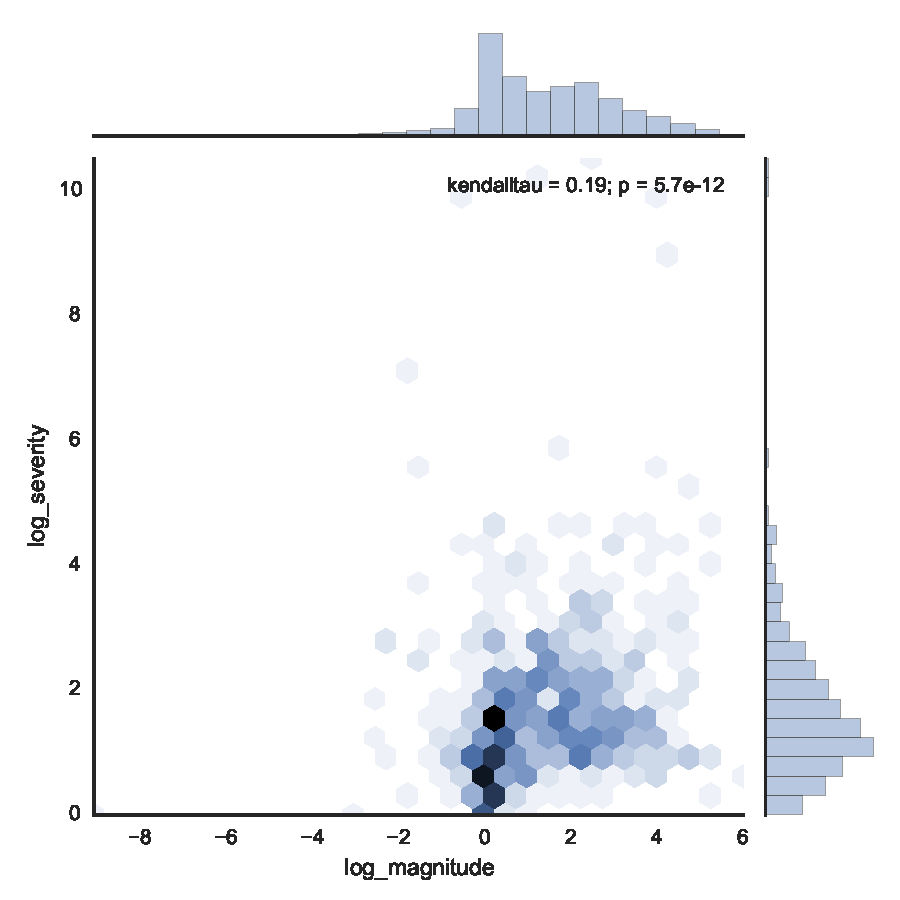
\includegraphics[width=\columnwidth]{log_magnitude_log_severity}
\caption{The relative distribution of our dependent variables. Note that the magnitude is shown in terms of its natural log due to its heavy-tailed distribution. Both outcome measures exhibit a heavy-tailed non-normal distribution which is a violation of simple OLS assumptions. For this reason, our analysis uses a robust regression method using Huber weights.}
\end{figure}